% Introduction chapter text
\chapter{Introduction}
\label{Ch1}
\raggedbottom
\clearpage

\section{Rivers: The intersection of Earth's two carbon cycles}

On timescales ranging from decades to millions of years, Earth's climate and habitability are governed by a delicate balance between the production and consumption of atmospheric carbon dioxide (\ce{CO2}). Geologic processes such as metamorphic outgassing \citep{Becker:2008bd}, volcanism \citep{Marty:1998vo}, rock weathering \citep{Walker:1981wn}, and subduction of marine sediments \citep{Kelemen:2015ec} act as a net source or sink of \ce{CO2} to Earth's surface, thus regulating the size and redox state of the surface carbon reservoir \citep{Hayes:2006ca}. On shorter timescales, the mass of carbon contained in the atmosphere as \ce{CO2} (reported in partial pressure, \textit{p}\ce{CO2}) is largely determined by an intricate network of sources and sinks that shuttle carbon between terrestrial reservoirs such as vegetation and soils, the ocean, and marine sediments \citep[collectively termed the "biosphere";][]{Sarmiento:2006wz}. By integrating multiple carbon sources on terrestrial landscapes and transferring this material to coastal margins, rivers offer a direct link between the geologic and biospheric carbon cycles (Figure \ref{Ch1Fig:1}). Furthermore, the ability of rivers to transfer carbon between these reservoirs is governed by a combination of climatic (\textit{e.g.} precipitation) and tectonic (\textit{e.g.} mountain uplift) controlling mechanisms \citep{Molnar:1990um}. Fluvial processes act as both a driver of and a response to global carbon cycle perturbations, and therefore uniquely describe the dynamic intersection between Earth's two carbon cycles.

% Figure 1
\begin{figure}[h]
	\makebox[\textwidth][c]{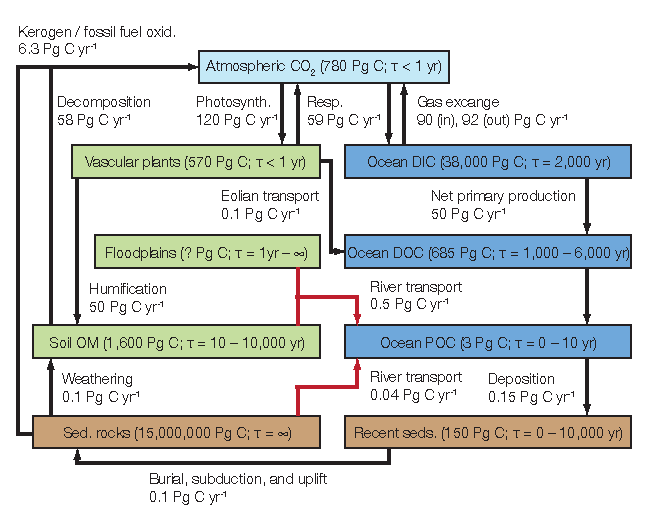
\includegraphics[]{Thesis_Figures/Ch1Fig1}}
	\caption[Carbon cycle reservoir inventories and fluxes]{Estimates of major reservoir inventories (in PgC; $1$ PgC = $10^{15}$ gC) and carbon fluxes (in PgC yr\textsuperscript{-1}). Box colors correspond to the following reservoir types: light blue, atmosphere; dark blue, marine; green, terrestrial; brown, geologic. Figure modified from \citet{Bianchi:2011cu}.}
	\label{Ch1Fig:1}
\end{figure}

\subsection{The biospheric carbon cycle}

The major mechanism by which carbon is transferred between biospheric reservoirs is the fixation of \ce{CO2} to biomass via photosynthesis and the corresponding respiration of organic matter back to \ce{CO2}:

% Equation 1
\begin{equation}\label{Ch1Eq:1}
	\ce{CO2 + H2O <=>[{photosynthesis}][{respiration}] CH2O + O2}
\end{equation}

where \ce{CH2O} represents organic carbon contained in biomass (OC\textsubscript{bio}). Globally, if photosynthesis outpaces respiration, then this process results in a net increase in the size of surficial OC reservoirs and therefore a decrease in \textit{p}\ce{CO2}, while the opposite is also true. However, it is well known that the biosphere is nearly entirely self-contained, resulting in a near-perfect balance between photosynthetic \ce{CO2} fixation and subsequent respiration on a global scale \citep{Sarmiento:2006wz}. Despite this, small imbalances do persist, resulting in a "leaky" biosphere and the accumulation of OC\textsubscript{bio} within marine sediments (Figure \ref{Ch1Fig:1}).

One process by which sedimentary OC accumulation can occur is the erosion of terrestrial landscapes and transport of particulate OC (POC) to coastal margin sediments via rivers \citep{Ludwig:1996ul,Schlunz:2000tl}. Although fluvial POC export flux represents only a small fraction of terrestrial net primary production \citep[\textit{i.e.} $\leq 1$\%;][]{Galy:2015fx}, this process continuously removes OC from the terrestrial biosphere that could have otherwise been respired. If this material subsequently escapes remineralization in marine sediments, as has been observed in many fluvial fan settings \citep{Derry:1996um,Burdige:2005tr,Galy:2007ev,Hilton:2008fo}, then riverine POC transport can constitute a quantitatively important atmospheric \ce{CO2} sink over geologic timescales. 

Because fluvial suspended sediment and POC fluxes are known functions of hydrology and river discharge \citep{Milliman:2011ug}, which is itself controlled by precipitation patterns \citep[\textit{e.g.}][]{Jian:2009bz}, this process describes a direct response of the carbon cycle to changing climate -- that is, riverine carbon export constitutes a climate feedback. Furthermore, POC yield depend on the rate at which river networks are able erode the landscape \citep{Ludwig:1996ul,Ludwig:1998ud,Galy:2015fx}. In addition to climatic factors, erosion rates strongly depend on geologic variables such as lithology, landscape slope, and tectonic uplift rate \citep{Dadson:2003kl,Milliman:2011ug,Hilton:2016dz}. Fluvial POC export therefore represents the intersection between hydrologic and geologic carbon cycle controls. However, the relative responses to changes in such controls remain largely elusive, hindering our ability to quantitatively reconstruct the role of fluvial climate feedbacks in the past and to predict future changes.

% Figure 2
\begin{figure}[t]
	\makebox[\textwidth][c]{\includegraphics[]{Thesis_Figures/Ch1Fig2}}
	\caption[Schematic representation of Earth's two carbon cycles]{Schematic interpretation of the two carbon cycles, including the hypothesized governing climatic and geologic mechanisms. Credit: Eric Taylor, WHOI Graphics Services.}
	\label{Ch1Fig:2}
\end{figure}

\subsection{The geologic carbon cycle}

In addition to the transport and burial of OC\textsubscript{bio}, highly erosive river networks draining meta-sedimentary lithologies incorporate a significant amount of rock-derived OC \citep[OC\textsubscript{petro}; \textit{e.g.}][]{Hilton:2011jw,Galy:2015fx}. Because they integrate the slowly subducted and lithified marine sediments on timescales of millions to tens of millions of years (Figure \ref{Ch1Fig:2}), meta-sedimentary rocks represent the largest global OC stock by nearly $3$ orders of magnitude (Figure \ref{Ch1Fig:1}). While the vast majority of this reservoir is effectively decoupled from surface processes on shorter timescales, respiration of exposed OC\textsubscript{petro} during fluvial transit represents an atmospheric \ce{CO2} source \citep{Galy:2008ff,Bouchez:2010if,Hilton:2014dh}. Because OC\textsubscript{petro} available for weathering is roughly double that of atmospheric \ce{CO2} \citep[\textit{i.e.} 1100 PgC in the upper $1$ m;][]{Copard:2007bf}, even a small perturbation in oxidation rates could lead to large changes in the resulting atmospheric \ce{CO2} flux. 

While it is currently estimated that the fluvial OC\textsubscript{bio} export flux to the coastal ocean is $\approx 3\times$ greater than that of OC\textsubscript{petro} \citep{Galy:2015fx}, atmospheric \ce{CO2} emissions due to OC\textsubscript{petro} oxidation remains elusive \citep{Galy:2008ff,Bouchez:2010if,Hilton:2014dh}, largely due to the fact that the kinetic, environmental, and compositional controls on this flux are poorly constrained. For example, because there exist few measurements of oxidation rate constants \citep{Chang:1999vo}, it remains unknown if OC\textsubscript{petro} weathering is limited by erosion rates or kinetic constraints, while the roles of partial oxidation \citep{Schillawski:2008ko} and OC\textsubscript{petro} chemical composition \citep{Galy:2008ff} have additionally received little attention. Furthermore, the relative response of OC\textsubscript{bio} burial and OC\textsubscript{petro} oxidation to changing climatic and geologic processes is not fully understood. For example, it has been proposed that high runoff due to increased intensity and frequency of tropical storms during periods of elevated atmospheric \ce{CO2} should lead to increased export and burial of OC\textsubscript{bio}, thus lowering \ce{CO2} concentrations \citep[\textit{i.e.} a negative feedback loop;][]{Hilton:2008fo}. However, high runoff has also been shown to result in elevated sediment yield and denudation rates, thus increasing the exposure of freshly uplifted OC\textsubscript{petro} to weathering and resulting in a positive feedback \citep{Hilton:2014dh}.

Still, the net effect of OC incorporation, transport, and evolution within fluvial systems on \textit{p}\ce{CO2} must reflect the balance between: \textit{(i.)} burial of recently fixed OC\textsubscript{bio} and \textit{(ii.)} oxidation of eroded OC\textsubscript{petro} (Figure \ref{Ch1Fig:2}). Constraining the response these two processes to both climatic and geologic perturbations is therefore a major motivating factor for this thesis.

\section{Motivation for this work}

\subsection{Constraining feedback mechanisms}

While critically important for understanding the global carbon cycle, quantifying modern fluvial fluxes alone (Figure \ref{Ch1Fig:1}) does not offer insight into the governing mechanisms that control OC source, transport, and fate. On the global scale, the importance of constraining such feedback mechanisms has long been recognized in order to reconstruct changes in atmospheric \ce{CO2} concentration over geologic timescales \citep{Berner:1999wj}. However, this has only recently been applied to modern fluvial systems. For example, recent studies \citep[\textit{e.g.}][]{Hilton:2008fo,Hilton:2012dt,Galy:2015fx} highlight the importance of erosive processes and sediment yield in determining both OC\textsubscript{bio} and OC\textsubscript{petro} export fluxes, suggesting that increased storm-driven erosion due to elevated \ce{CO2} concentrations could provide a negative feedback by increasing OC\textsubscript{bio} burial in marine sediments.

Furthermore, it is now known that OC transport through river networks is not passive. Rather, fluvial transit integrates the complex interactions between multiple biogeochemical processes, each of which has the ability to alter the evolution of OC quality and quantity \citep{Cole:2007gp,Aufdenkampe:2011fm,Bianchi:2011cu}. This has lead to a new paradigm in our understanding of passive-margin systems in which OC is continuously deposited, chemically altered, and resuspended during transit \citep[the so-called "river continuum"; Figure \ref{Ch1Fig:3};][]{Blair:2012du}. In contrast, active-margin systems are now recognized not only as regions of intense erosion and OC\textsubscript{bio} export, but also for OC\textsubscript{petro} weathering due to uplift of OC-rich meta-sedimentary rocks \citep[Figure \ref{Ch1Fig:3};][]{Milliman:1992fu}. Therefore, based on this current understanding, passive-margin and active-margin systems are expected to respond to environmental perturbations in fundamentally unique ways.

This thesis aims to advance our mechanistic understanding of fluvial carbon cycle feedbacks. To do so, I compare two end-member systems: \textit{(i.)} the Congo River representing large, floodplain-dominated, and low-erosion environments in order to isolate climatic controls; and \textit{(ii.)} rivers draining the highly erosive Central Range of Taiwan in order to determine geologic controls on active margins.

% Figure 3
\begin{figure}[t]
	\makebox[\textwidth][c]{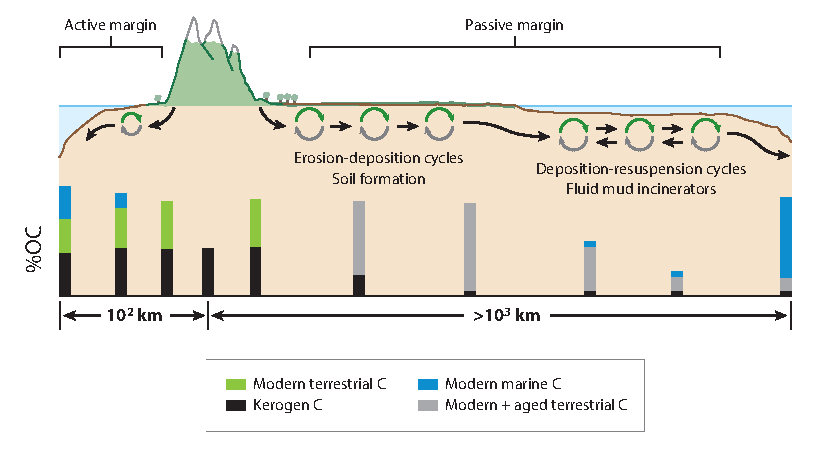
\includegraphics[]{Thesis_Figures/Ch1Fig3}}
	\caption[Schematic representation of the river continuum]{Schematic representation of fluvial particulate OC evolution in passive-margin and active-margin systems. Figure modified from \citet{Blair:2012du}.}
	\label{Ch1Fig:3} 
\end{figure}

\subsection{The need for time-series measurements}

Fluvial systems are inherently dynamic in nature. However, there exist surprisingly few studies that consider riverine carbon export in a time-series manner, especially when including suspended sediments and particulate OC. Although such studies are logistically difficult, they provide critically important information regarding the seasonal variability and long-term evolution of river basins \citep[\textit{e.g.}][]{Peterson:2002hj,Raymond:2003fd,Milliman:2011ug,Voss:2015dd}. In addition to refining our estimates of carbon flux (Figure \ref{Ch1Fig:1}), time-series measurements have revealed that OC composition exhibits significant temporal variability that is related to hydrology \citep{Voss:2015dd,Hemingway:2016bq}. Furthermore, time-series studies provide a necessary link between the synoptic, "campaign-style" results that describe most of our knowledge on modern river systems with paleoclimate reconstructions utilizing sediments deposited in river-dominated margins. In this thesis, I attempt to further develop this emerging "time-variable river continuum" model by utilizing a 34-month time-series of monthly measurements on the Congo River in addition to a high-resolution (sub-daily) sampling scheme across three successive typhoon events in Taiwan. 

\subsection{Current methodological limitations}

Currently, most studies aimed at constraining the source and composition of exported fluvial OC utilize the following techniques: \textit{(i.)} conservative tracers of bulk OC composition (\textit{e.g.} \ce{^{14}C} content, \ce{^{13}C} content, N/C ratios, \textit{etc.}); \textit{(ii.)} compound-specific biomarker concentrations and isotope composition (\textit{e.g.} \textit{n}-alkyl lipds, sterols, lignin oxidation products); and \textit{(iii.)} high-resolution non-quantitative mass spectrometry. When used in tandem, these techniques offer a powerful approach to understanding OC sources. 

However, each comes with its own drawbacks. For example, bulk measurements provide a weighted-average view of the composition of all OC contained within a sample, but require \textit{a priori} knowledge of end-member compositions in order to un-mix source contributions \citep{Perdue:2007fn,Weijers:2009iu,Hilton:2010cg,Hossler:2012jh}. In contrast, biomarker concentration and isotope measurements provide information specific to a particular OC source, but individual compounds typically constitute $\leq 1$\% of total OC and are subject to potentially large and unknown production biases \citep{Garcin:2014hg,Ponton:2014jr}. To address these drawbacks, a 4\textsuperscript{th} class of organic geochemical techniques is emerging -- reaction monitoring methods \citep[\textit{e.g.}][]{Rosenheim:2008ed,Follett:2014if,Beaupre:2016km}. In addition to geochemical applications using time-series fluvial sediments, this thesis aims to advance our theoretical understanding of one such reaction monitoring technique, specifically the "Ramped PyrOx" (RPO) serial oxidation method. By heating a sample at a constant ramp rate and "binning" evolved \ce{CO2} for isotope measurements, this technique directly relates OC (thermo-)lability and isotope composition, and is therefore a promising method for monitoring OC degradation kinetics in the environment and for un-mixing OC sources.

\subsection{Thesis outline}

This thesis is motivated by a set of questions that aim to further our understanding of the environmental processes governing the role of rivers in the global carbon cycle. Thematically, these questions can be separated into two main sections:

\begin{enumerate}
\item \textbf{Ramped pyrolysis/oxidation (RPO) instrumental development, theory, data treatment, and post-processing} (Chapters \ref{Ch2} and \ref{Ch3}).
	\begin{itemize}
	\item What is the contribution by contaminant ("blank") carbon in the RPO instrument, and how can this be corrected for? Does the RPO instrument impart any isotope fractionation?
	\item Can profiles of organic carbon thermal recalcitrance be related to intrinsic molecular properties, and what are the governing kinetic reactions?
	\item How can RPO-derived thermal profiles and isotope results be combined to advance our understanding of organic carbon sources and processing in the environment?  
	\end{itemize}
\item \textbf{Application of organic geochemical methods to riverine suspended sediments and soils} (Chapters \ref{Ch4}, \ref{Ch5}, and \ref{Ch6}).
	\begin{itemize}
	\item How do the signals recorded in the fluvially exported particulate organic carbon integrate processes throughout the basin? Are they representative of upstream sources?
	\item Do these signals respond to environmental variability (\textit{e.g.} hydrology, temperature) on seasonal and inter-annual timescales? How does this knowledge affect our interpretation of paleoenvironmental reconstructions using sedimentary archives?
	\item How would changes in environmental conditions affect the stability of carbon reservoirs (\textit{e.g.} soils, rock-derived organic carbon) and the corresponding \ce{CO2} flux from these reservoirs to the atmosphere?
	\end{itemize}
\end{enumerate}

In practice, this thesis is articulated around the following chapters:

\subsubsection{Chapter 2}

This chapter describes recent developments to the RPO radiocarbon instrument located at the National Ocean Sciences Accelerator Mass Spectrometer (NOSAMS) facility. This method aims to separate individual components contained within complex OC mixtures based on thermo-lability and to evaluate the range of both stable carbon (\ce{^{13}C} and \ce{^{12}C}) and radiocarbon (\ce{^{12}C}) composition contained within a given sample. Here, the contribution and isotope composition of contaminant ("blank") carbon is constrained and equations are presented to correct for this. Additionally, the isotope fractionation due to mass-balance effects is determined based on a compilation of 66 samples that have been analyzed over $\approx 4$ years, while the fractionation due to kinetic effects is evaluated using a set of standard reference materials. 

\subsubsection{Chapter 3}

Here, a framework in which to interpret RPO isotope and kinetic results is proposed. OC decomposition kinetics are described as a continuous superposition of parallel first-order decay reactions that are governed by the Arrhenius equation. The distribution of activation energy required to explain observed thermal profiles is then constrained by solving the regularized inverse problem, thus relating RPO experimental results with intrinsic chemical properties of a given sample. To robustly verify the assumptions built into this model, a set of test samples was analyzed under a range of experimental conditions. Lastly, this chapter discusses how the RPO instrument presents a novel approach for separating carbon sources and understanding OC transformation processes.

\subsubsection{Chapter 4}

This chapter concerns the seasonal and inter-annual variability of vascular-plant-derived biomarker concentrations and $\delta^{13}$C values exported from the Congo River. Changes in the composition of vascular plant lipids (\textit{n}-alkanes, \textit{n}-alcohols, and \textit{n}-alkanoic acids) extracted from fluvial sedimentary archives are commonly used as a tracer for changes in past ecosystem structure carbon export. However, few studies have monitored the role of inter-annual variability on these signals. Using a 34-month time-series collected from the Congo River at Brazzaville, this chapter shows that alkyl lipid compound classes variably track upstream ecosystems and that \textit{n}-alcohols and \textit{n}-alkanoic acids are more susceptible to seasonal variability than are \textit{n}-alkanes. 

\subsubsection{Chapter 5}

Using the same Congo River sample set, Chapter \ref{Ch5} constrains the source of exported particulate OC using bulk conservative tracers ($\delta^{13}$C, $\Delta^{14}$C, N/C) and microbial glycerol dialkyl glycerol tetraether (GDGT) biomarkers. Variability in OC sources is shown to be driven by inter-annual hydrodynamic variability, with exported OC being dominated by significantly pre-aged material eroded from the \textit{Cuvette Congolaise} swamp forest during periods of high northern-hemisphere discharge. Compared to published time-series data from an upstream tributary (Oubangui River), these results offer insight into the dilution and replacement of upstream POC by downstream sources during fluvial transit. Combined, Chapters \ref{Ch4} and \ref{Ch5} constrain the environmental processes governing Congo River OC export by highlighting the importance of seasonal and inter-annual hydrologic variability.

\subsubsection{Chapter 6}

Lastly, using a combination of bulk measurements, alkanoic acid biomarkers, and RPO results, this chapter reveals that the oxidation of rock-derived OC in the highly erosive Central Range of Taiwan is governed by microbial processes, a phenomenon that has previously been observed in laboratory incubation experiments but has yet to be verified as quantitatively important in the field. Additionally, the resulting \ce{CO2} flux to the atmosphere is constrained to be roughly equal to that of \ce{CO2} drawdown due to silicate weathering and burial of biospheric OC in this system. Because microbial oxidation appears to be rapid, it is likely not kinetically limited and resulting \ce{CO2} fluxes are governed by the rate of exposure of bedrock material to the weathering front (\textit{i.e.} erosion rate).
